\documentclass[10pt,twocolumn,a4paper]{article}

% ==========================================================================
% Pacotes Padrão (100% compatíveis com Overleaf / TeX Live)
% Observação: Caso o template específico do Prof. Wagner utilize um .cls/.sty
% próprio, basta substituir o preâmbulo mantendo as seções abaixo.
% ==========================================================================
\usepackage[utf8]{inputenc}
\usepackage[T1]{fontenc}
\usepackage[brazil]{babel}
\usepackage{newtxtext,newtxmath} % Tipografia estilo ACM/IEEE (Times)
\usepackage[margin=1.8cm,columnsep=0.75cm]{geometry}
\usepackage{graphicx}
\usepackage{booktabs}
\usepackage{multirow}
\usepackage{amsmath}
\usepackage{algorithm}
\usepackage{algpseudocode}
\usepackage{listings}
\usepackage{xcolor}
\usepackage{caption}
\usepackage{subcaption}
\usepackage[colorlinks=true,linkcolor=blue!60!black,citecolor=blue!60!black,urlcolor=blue!60!black]{hyperref}

\graphicspath{{./figures/}}

\lstdefinestyle{cppstyle}{
    language=C++,
    basicstyle=\ttfamily\scriptsize,
    keywordstyle=\color{blue!75!black}\bfseries,
    commentstyle=\color{green!50!black}\itshape,
    stringstyle=\color{red!60!black},
    numbers=left,
    numberstyle=\tiny\color{gray},
    stepnumber=1,
    numbersep=5pt,
    frame=single,
    breaklines=true,
    tabsize=2,
    showstringspaces=false
}

% ==========================================================================
% Metadados do Artigo
% ==========================================================================
\title{\textbf{Modelagem e Simulação Procedural de Rios Meândricos com Modulação Espacial por Mobilidade Litológica Relativa}}

\author{
    Alberto Henrique \quad Pedro Henrique Braga \quad Warley Ramires \\[0.3em]
    \small Orientador: Prof. Dr. Wagner Ferreira de Barros \\
    \small Curso de Bacharelado em Ciência da Computação -- Instituto Federal do Norte de Minas Gerais (IFNMG) \\
    \small Disciplina de Computação Gráfica (2026/2)
}

\date{Novembro de 2026}

\begin{document}

\maketitle

% ==========================================================================
% Resumo & Abstract
% ==========================================================================
\begin{abstract}
\noindent
A síntese procedural de redes hidrográficas e planícies aluviais é um problema central na modelagem de terrenos virtuais em Computação Gráfica. Métodos recentes baseados em curvas paramétricas, como o modelo proposto por Paris et al. (SIGGRAPH Asia 2023), simulam com alta eficiência a migração lateral, o corte de meandros (\textit{cutoffs}) e eventos de avulsão em escala de dezenas de quilômetros. Contudo, a formulação original assume uma erodibilidade lateral uniforme ao longo do substrato, modulando o deslocamento apenas pela declividade topográfica e por restrições pontuais de autoria. Neste trabalho, investigamos e implementamos uma extensão geomorfológica leve que introduz um campo escalar bidimensional independente de mobilidade litológica relativa $E(x,y)$, amostrado diretamente na margem externa (\textit{cut bank}) do canal fluvial a uma distância de meia largura em relação à linha central. O fator de mobilidade normalizado $g(E) = \text{clamp}(E / \bar{E}, g_{\min}, g_{\max})$ atua multiplicativamente sobre a taxa cinemática de migração, permitindo simular desde barreiras rochosas resistentes ($E < \bar{E}$) até depósitos sedimentares friáveis ($E > \bar{E}$). Validamos a implementação por meio de testes de regressão numérica sob substrato homogêneo (erro $L_\infty \le 10^{-9}$ em relação à \textit{baseline} oficial) e avaliamos o impacto de heterogeneidades litológicas na trajetória, na sinuosidade temporal $S(t)$, no comprimento de onda $\lambda$, na ocorrência de \textit{cutoffs} e no custo computacional por passo de simulação.

\vspace{0.5em}
\noindent\textbf{Palavras-chave:} Computação Gráfica, Modelagem Procedural de Terrenos, Rios Meândricos, Mobilidade Litológica, Simulação Fluvial.
\end{abstract}

% ==========================================================================
% 1. Introdução
% ==========================================================================
\section{Introdução}
\label{sec:introducao}

A geração realista de terrenos virtuais é um requisito essencial em jogos eletrônicos, simuladores de treinamento, cinema e visualização científica. Enquanto técnicas clássicas baseadas em ruído coerente (como Perlin ou Simplex) produzem relevos montanhosos plausíveis a baixo custo, elas falham em capturar a estrutura espacial e a evolução temporal de sistemas fluviais, especialmente em planícies aluviais dominadas por rios meândricos. No extremo oposto, simulações físicas baseadas em dinâmica dos fluidos computacional (CFD) tridimensional ou equações de águas rasas acopladas ao transporte de sedimentos apresentam custo computacional proibitivo para domínios extensos e fluxos de trabalho interativos de autoria.

Para conciliar realismo geomorfológico, controle artístico e desempenho, Paris et al.~\cite{paris2023meandering} introduziram no SIGGRAPH Asia 2023 um arcabouço cinemático-geométrico para autoria e simulação de rios meândricos. O método representa os canais como curvas paramétricas discretizadas cujos vértices migram lateralmente com base na curvatura local e na convolução ponderada das curvaturas a montante (\textit{upstream}), fundamentando-se nos modelos clássicos da geomorfologia fluvial de Ikeda et al.~\cite{ikeda1981bend} e Howard e Knutson~\cite{howard1984sufficient}.

Apesar de considerar a atenuação da migração pela declividade do terreno ($\nabla h$) e por restrições de controle do usuário, a implementação de referência assume que o substrato geológico possui erodibilidade lateral uniforme em todo o domínio. Na natureza, entretanto, planícies fluviais frequentemente interceptam unidades litológicas distintas --- como intrusões rochosas resistentes, terraços consolidados ou lentes de sedimentos inconsolidados --- que restringem ou aceleram localmente a erosão da margem externa (\textit{cut bank}), gerando meandros confinados e assimétricos.

\subsection{Questão de Investigação e Hipóteses}
Este trabalho investiga a seguinte questão de pesquisa:
\begin{quote}
\textit{``Como a introdução de uma matriz bidimensional de mobilidade litológica relativa $E(x,y)$, independente da topografia e amostrada na margem externa do canal, modula a taxa de migração lateral, a morfometria (sinuosidade e comprimento de onda) e a estabilidade numérica de rios meândricos procedurais?''}
\end{quote}

Formulamos duas hipóteses principais:
\begin{enumerate}
    \item \textbf{Hipótese Morfométrica:} Regiões de menor mobilidade litológica ($E < \bar{E}$, rochas resistentes) atenuarão localmente a migração lateral da margem externa, deformando a simetria das alças meândricas e retardando ou deslocando espacialmente a ocorrência de \textit{cutoffs} topológicos.
    \item \textbf{Hipótese de Desempenho e Compatibilidade:} A consulta bilinear na margem externa adicionará sobrecarga computacional inferior a $5\%$ na mediana do tempo por passo de simulação e preservará paridade numérica exata ($L_\infty \le 10^{-9}$) com a \textit{baseline} quando $E(x,y)$ for uniforme.
\end{enumerate}

% ==========================================================================
% 2. Trabalho de Referência e Fundamentação
% ==========================================================================
\section{Trabalho de Referência e Fundamentação}
\label{sec:fundamentacao}

No método de Paris et al.~\cite{paris2023meandering}, cada canal fluvial é representado por uma sequência ordenada de pontos bidimensionais $\mathbf{p}_i \in \mathbb{R}^2$ ($i = 0, \dots, N-1$) com largura $w$ e profundidade $d$, reamostrados uniformemente a cada passo de tempo $\Delta t$ segundo uma distância de amostragem $\Delta s$.

\subsection{Taxa de Migração na Baseline}
Para cada vértice $\mathbf{p}_i$, define-se a taxa de migração local $R_0(i)$ proporcional à curvatura escalada do canal:
\begin{equation}
    R_0(i) = k_1 \cdot w \cdot C(i),
    \label{eq:local_migration}
\end{equation}
onde $k_1$ é a constante de migração cinemática e $C(i)$ é a curvatura discreta assinada no ponto $\mathbf{p}_i$. Para reproduzir o atraso espacial entre a curvatura do canal e a velocidade máxima junto à margem (que causa a translação dos meandros para jusante), a taxa efetiva $\mu_{\text{base}}(i)$ combina a curvatura local com uma convolução exponencial das taxas a montante ao longo da distância curvilinear $s$:
\begin{equation}
    \mu_{\text{base}}(i) = \sigma^{-2/3} \left( \Omega R_0(i) + \Gamma \frac{\sum_{k \ge 0} R_0(i-k) \, G(k)}{\sum_{k \ge 0} G(k)} \right),
    \label{eq:total_migration}
\end{equation}
em que $\sigma$ é a sinuosidade global do canal, $\Omega = -1.0$ e $\Gamma = 2.5$ são constantes de ponderação geomorfológica, e $G(k) = \exp(-\alpha \, s_{i, i-k})$ é o núcleo de decaimento exponencial com $\alpha = 2 k C_f / d$.

O deslocamento lateral do ponto $\mathbf{p}_i$ no passo $\Delta t$ é então dado por:
\begin{equation}
    \mathbf{p}_i(t + \Delta t) = \mathbf{p}_i(t) + w_f(i) \, w_t(i) \, \Delta t \, \mu_{\text{base}}(i) \, \mathbf{d}_{\text{mig}}(i),
    \label{eq:baseline_step}
\end{equation}
onde $w_f(i)$ é o fator de amortecimento nas extremidades do canal, $w_t(i)$ é o amortecimento imposto pela declividade topográfica $\|\nabla h(\mathbf{p}_i)\|^2$, e $\mathbf{d}_{\text{mig}}(i)$ é a direção normal de migração (combinada com eventuais restrições autorais).

\begin{figure}[t]
    \centering
    \begin{subfigure}[b]{0.48\columnwidth}
        \centering
        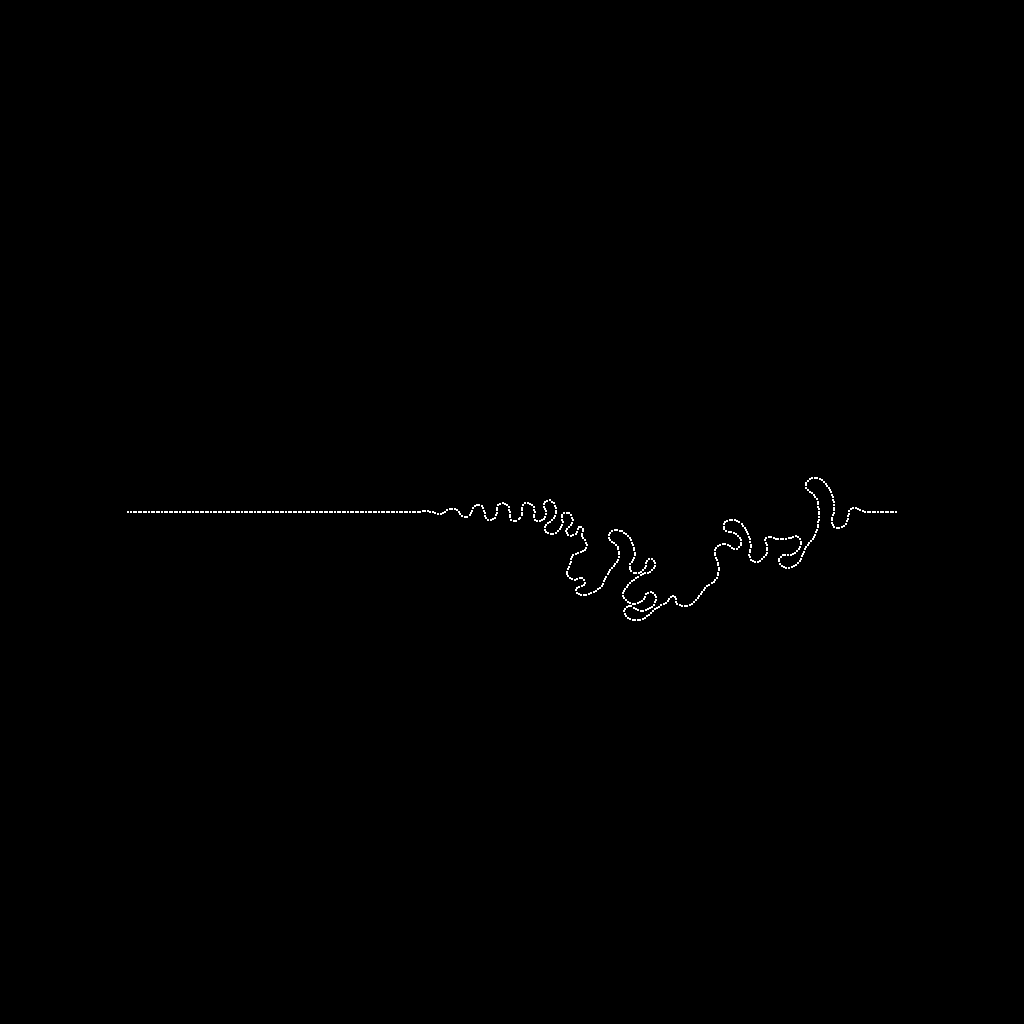
\includegraphics[width=\textwidth]{meander_simple.png}
        \caption{Canal em terreno plano ($500$ passos).}
        \label{fig:baseline_simple}
    \end{subfigure}
    \hfill
    \begin{subfigure}[b]{0.48\columnwidth}
        \centering
        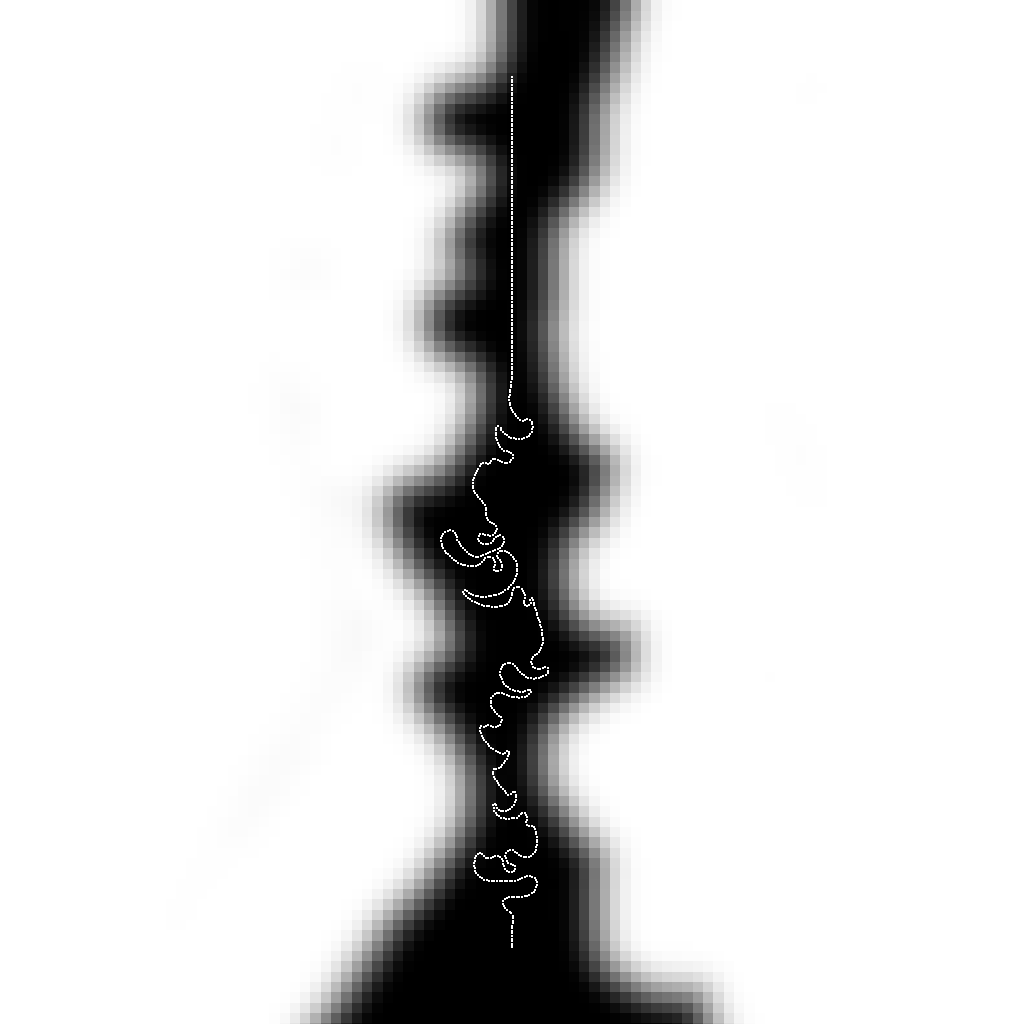
\includegraphics[width=\textwidth]{meander_terrain.png}
        \caption{Canal restrito por relevo ($1200$ passos).}
        \label{fig:baseline_terrain}
    \end{subfigure}
    \caption{Exemplos reproduzidos a partir do código público de referência (\textit{baseline}) de Paris et al.~\cite{paris2023meandering}.}
    \label{fig:baseline_examples}
\end{figure}

% ==========================================================================
% 3. Proposta: Modulação por Mobilidade Litológica Relativa
% ==========================================================================
\section{Modulação por Mobilidade Litológica Relativa}
\label{sec:proposta}

Embora a Equação~\eqref{eq:baseline_step} considere o gradiente de elevação $w_t(i)$, uma planície aluvial com declividade suave ($\|\nabla h\| \approx 0 \Rightarrow w_t(i) \approx 1$) pode apresentar variações expressivas na coesão e resistência litológica do substrato. Nossa proposta introduz um campo escalar 2D independente $E(x,y) \ge 0$, representado por uma estrutura \texttt{ScalarField2D} que pode ser gerada proceduralmente ou carregada a partir de um mapa em escala de cinza.

\subsection{Amostragem na Margem Externa (\textit{Cut Bank})}
Fisicamente, a migração lateral decorre da erosão fluvial concentrada na margem côncava (externa) da curva. Em vez de amostrar o campo $E(x,y)$ na linha central $\mathbf{p}_i$, calculamos a posição da margem externa $\mathbf{x}_{\text{bank}}(i)$ deslocando o ponto central por meia largura ($w/2$) na direção determinada pelo sinal da curvatura local $C(i)$:
\begin{equation}
    \mathbf{x}_{\text{bank}}(i) = \mathbf{p}_i + \boldsymbol{\delta}_{\text{ext}}(i), \quad
    \boldsymbol{\delta}_{\text{ext}}(i) =
    \begin{cases}
        -\frac{w}{2} \mathbf{n}_i, & \text{se } C(i) > \varepsilon_\kappa, \\
        +\frac{w}{2} \mathbf{n}_i, & \text{se } C(i) < -\varepsilon_\kappa, \\
        \mathbf{0}, & \text{se } |C(i)| \le \varepsilon_\kappa,
    \end{cases}
    \label{eq:cut_bank_offset}
\end{equation}
onde $\mathbf{n}_i$ é o vetor unitário ortogonal à tangente em $\mathbf{p}_i$ e $\varepsilon_\kappa = 10^{-12}$ define a zona de inflexão. Nos pontos de inflexão ($|C(i)| \le \varepsilon_\kappa$), consultamos ambas as margens ($\mathbf{p}_i \pm \frac{w}{2}\mathbf{n}_i$) por interpolação bilinear e utilizamos a média aritmética das amostras válidas.

\subsection{Normalização e Limitação (\textit{Clamping})}
Para garantir que qualquer campo uniforme $E(x,y) = c > 0$ seja estritamente neutro em relação à \textit{baseline}, o valor amostrado $E_{\text{sel}}(i)$ é normalizado pela média espacial $\bar{E}$ do campo litológico e limitado ao intervalo $[g_{\min}, g_{\max}] = [0.25, 2.0]$:
\begin{equation}
    g_i = \text{clamp}\left( \frac{E_{\text{sel}}(i)}{\bar{E}}, \, g_{\min}, \, g_{\max} \right).
    \label{eq:mobility_factor}
\end{equation}

A equação de atualização do vértice passa a ser:
\begin{equation}
    \mathbf{p}_i(t + \Delta t) = \mathbf{p}_i(t) + w_f(i) \, w_t(i) \, g_i \, \Delta t \, \mu_{\text{base}}(i) \, \mathbf{d}_{\text{mig}}(i).
    \label{eq:modified_step}
\end{equation}
Desse modo:
\begin{itemize}
    \item $E_{\text{sel}}(i) < \bar{E} \implies g_i < 1$: substrato resistente (ex.: rocha sã ou argila compactada), reduzindo a migração lateral;
    \item $E_{\text{sel}}(i) > \bar{E} \implies g_i > 1$: substrato friável/erodível (ex.: aluvião arenoso), acelerando a migração lateral;
    \item $E_{\text{sel}}(i) = \bar{E} \implies g_i = 1$: comportamento idêntico ao modelo original.
\end{itemize}

% ==========================================================================
% 4. Aspectos de Implementação
% ==========================================================================
\section{Aspectos de Implementação}
\label{sec:implementacao}

A extensão foi integrada de forma não intrusiva sobre o repositório oficial em C++17 (\texttt{aparis69/Meandering-rivers}, commit \texttt{f5a8ef3}). A Tabela~\ref{tab:arquivos_modificados} sintetiza os módulos modificados pela equipe.

\begin{table}[htbp]
    \centering
    \caption{Resumo dos arquivos alterados e adicionados em relação à \textit{baseline}.}
    \label{tab:arquivos_modificados}
    \footnotesize
    \begin{tabular}{p{0.36\columnwidth} p{0.56\columnwidth}}
        \toprule
        \textbf{Arquivo} & \textbf{Modificação / Responsabilidade} \\
        \midrule
        \texttt{Include/basics.h} & Adição do método \texttt{ScalarField2D::Mean()} para cálculo de $\bar{E}$. \\
        \texttt{Include/meanders.h} & Novos atributos \texttt{lithology}, \texttt{lithologyMean}, \texttt{lithologyEnabled} e sobrecarga de \texttt{Channel::Migrate()}. \\
        \texttt{Source/meanders-simulation.cpp} & Gerenciamento \textit{opt-in} do campo litológico e despacho condicional em \texttt{MigrateAllChannels()}. \\
        \texttt{Source/meanders-channel.cpp} & Amostragem bilinear na margem externa, tratamento de pontos de inflexão e aplicação de $g_i$. \\
        \texttt{Source/main.cpp} & Carregamento de mapas litológicos via \texttt{stb\_image.h} e cena de demonstração. \\
        \texttt{Tests/lithology\_regression.cpp} & Suite de regressão ($E=1$), validação de efeito em campo heterogêneo e verificação de \texttt{NaN}. \\
        \bottomrule
    \end{tabular}
\end{table}

Quando nenhum campo litológico é fornecido ao construtor de \texttt{MeanderSimulation}, a flag \texttt{lithologyEnabled} permanece falsa e o simulador executa exatamente o método original \texttt{Channel::Migrate()} sem qualquer alteração numérica.

% ==========================================================================
% 5. Metodologia Experimental
% ==========================================================================
\section{Metodologia Experimental}
\label{sec:metodologia}

Para avaliar rigorosamente a extensão proposta sob condições equivalentes às da \textit{baseline}, estabelecemos um protocolo experimental em três estágios de ablação:

\begin{enumerate}
    \item \textbf{Cenário 1 -- Paridade e Regressão ($E(x,y) = 1.0$):} Verifica se a ativação do pipeline litológico com campo uniforme preserva a trajetória exata da \textit{baseline} após $N$ passos sob a mesma semente pseudoaleatória (\texttt{seed = 1234}).
    \item \textbf{Cenário 2 -- Contraste Litológico Bimodal / Barreira:} Domínio dividido em zonas de baixa mobilidade ($E = 0.25$) e alta mobilidade ($E = 1.75$), avaliando a contenção seletiva das alças meândricas e a formação assimétrica do canal.
    \item \textbf{Cenário 3 -- Mosaico Litológico Contínuo / Mapa de Entrada:} Avaliação com campos espaciais carregados por imagem em escala de cinza combinados à topografia.
\end{enumerate}

\subsection{Métricas de Avaliação}
\begin{itemize}
    \item \textbf{Erro Geométrico de Paridade ($L_\infty$):} $\max_i \|\mathbf{p}_i^{\text{lito}} - \mathbf{p}_i^{\text{base}}\|_2$ para $E(x,y)$ constante;
    \item \textbf{Sinuosidade Temporal $S(t)$:} Razão entre o comprimento curvilinear total do canal $L(t)$ e a distância euclidiana entre suas extremidades;
    \item \textbf{Comprimento de Onda ($\lambda$) e Amplitude:} Distância média entre pontos de inflexão consecutivos e desvio lateral máximo por zona litológica;
    \item \textbf{Eventos Topológicos (\textit{Cutoffs}):} Número e localização espacial dos estrangulamentos de meandros ao longo da simulação;
    \item \textbf{Desempenho Computacional:} Tempo de execução por passo (mediana e percentil 95 em milissegundos).
\end{itemize}

% ==========================================================================
% 6. Resultados Preliminares (Checkpoint 2)
% ==========================================================================
\section{Resultados Preliminares}
\label{sec:resultados}

Até o presente momento (Checkpoint 2), a implementação do núcleo de modulação litológica e a bateria de validação funcional foram concluídas e verificadas:

\begin{itemize}
    \item \textbf{Validação da Regressão ($E=1$):} O teste automatizado em \texttt{Tests/lithology\_regression.cpp} executa $50$ passos da \textit{baseline} e da versão com campo uniforme $256 \times 256$ ($E=1.0$), confirmando que todos os vértices do canal coincidem dentro da tolerância $\varepsilon = 10^{-9}$.
    \item \textbf{Sensibilidade a Campos Heterogêneos e Estabilidade:} No teste bimodal ($E = 0.25$ para $x < 0$ e $E = 1.75$ para $x \ge 0$), a trajetória diverge significativamente da \textit{baseline} ($> 10^{-6}$) mantendo $100\%$ dos vértices livres de valores inválidos (\texttt{NaN} ou infinito) após as etapas de migração, \textit{cutoff} e reamostragem cúbica.
\end{itemize}

\begin{figure}[htbp]
    \centering
    \begin{subfigure}[b]{0.48\columnwidth}
        \centering
        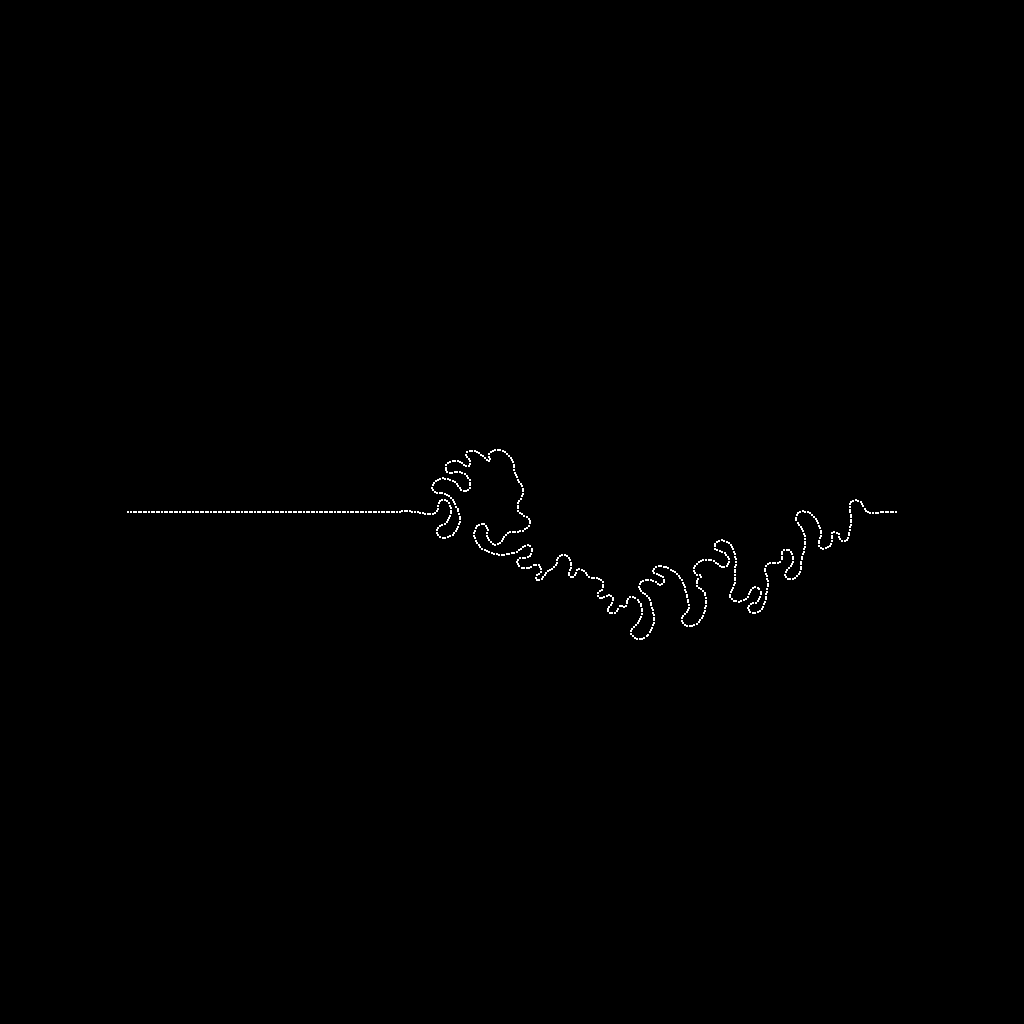
\includegraphics[width=\textwidth]{avulsion_before.png}
        \caption{Antes da avulsão (passo $700$).}
    \end{subfigure}
    \hfill
    \begin{subfigure}[b]{0.48\columnwidth}
        \centering
        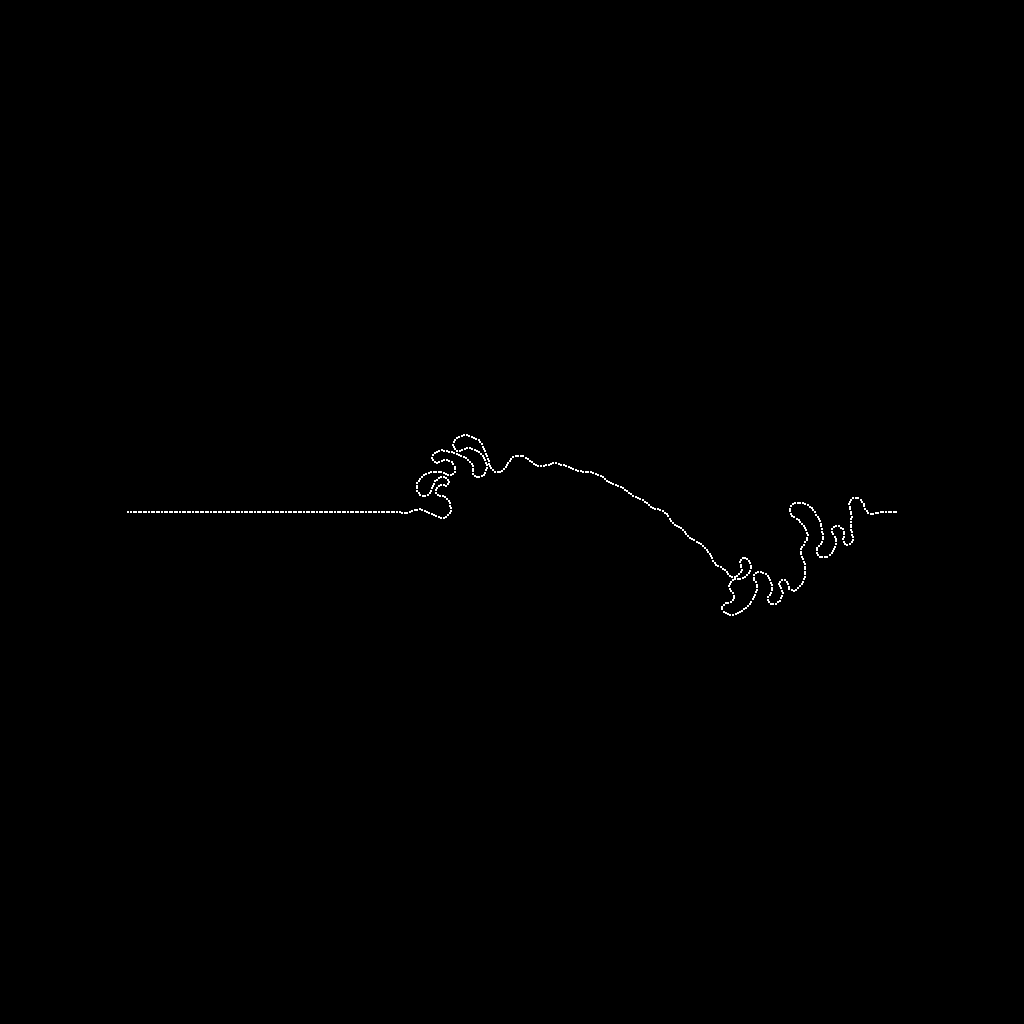
\includegraphics[width=\textwidth]{avulsion_after.png}
        \caption{Após avulsão e reamostragem.}
    \end{subfigure}
    \caption{Verificação dos operadores topológicos da \textit{baseline} (\textit{cutoffs} e avulsão) integrados ao pipeline.}
    \label{fig:avulsion_check}
\end{figure}

\noindent
\textit{[Nota para a versão final: As tabelas quantitativas de séries temporais de sinuosidade $S(t)$, contagem de cutoffs sob múltiplas sementes estocásticas e overhead de tempo de execução serão consolidadas nesta seção na próxima etapa do cronograma.]}

% ==========================================================================
% 7. Conclusões Parciais e Próximos Passos
% ==========================================================================
\section{Conclusões Parciais e Próximos Passos}
\label{sec:conclusao}

Este artigo em andamento apresentou a formulação e a implementação de um mecanismo de modulação espacial por mobilidade litológica relativa para simulação procedural de rios meândricos. A arquitetura implementada preserva total compatibilidade com o método de Paris et al.~\cite{paris2023meandering} e permite controlar a erodibilidade das margens externas de forma ortogonal à topografia.

Como plano objetivo para a conclusão até a entrega final, a equipe realizará: (i) a geração de mapas litológicos dedicados e visualização sobreposta das faixas de resistência nos arquivos de saída; (ii) a coleta automatizada das métricas quantitativas ($S(t)$, $\lambda$, \textit{cutoffs} e tempo por passo) com múltiplas sementes; e (iii) a discussão aprofundada dos resultados experimentais e limitações do modelo.

% ==========================================================================
% Referências Bibliográficas
% ==========================================================================
\bibliographystyle{plain}
\bibliography{referencias}

\end{document}
